\section{Technologies}\label{sec:technologies}
Before beginning the design of the system, a thorough analysis of the possible technologies are needed. 

\subsection{Protocol Layers}\label{sec:protocol-layers}
This section is based on the book ``Computer Networking: A Top Down Approach''~\citep[Chapter 1]{computer-networking}. The focus are on the five-layer Internet protocol stack (IP stack). The IP stack consists of five layers, Application, Transport, Network, Link, and Physical (Physical layer sometimes omitted).

The IP stack is not the only stack available, another popular stack is the ISO stack which consists of seven layers. These two stacks are similar as seen in \figref{fig:protocol-layers}. There are common layers in both of the stacks, which are arguably similar. The focus remains on the IP stack, as the additional layers the ISO stack does not provide any additional insight.

\begin{figure}[H]
     \center{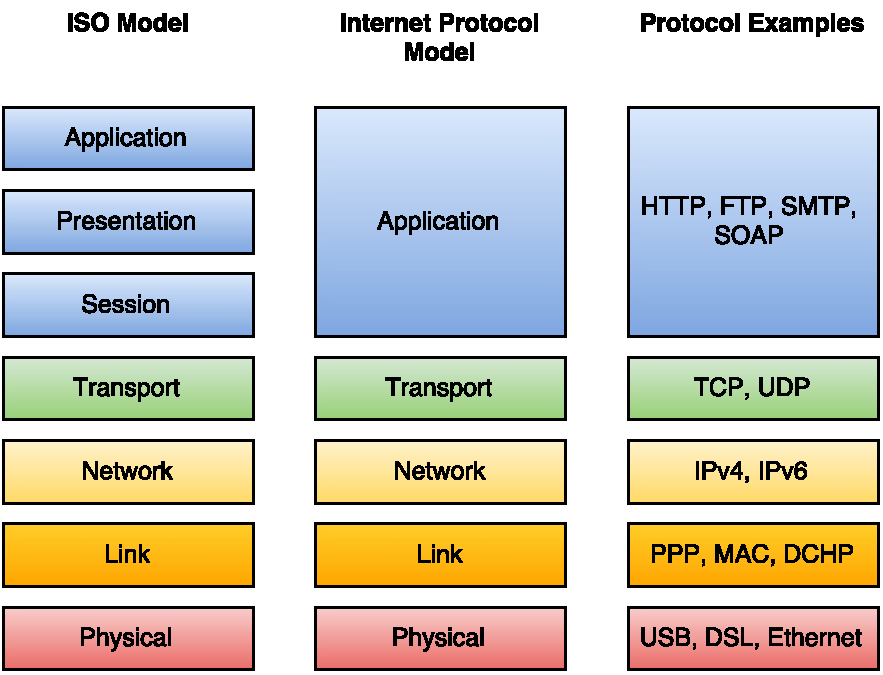
\includegraphics[width=\textwidth -100px]
     {graphics/protocol-layers.pdf}}
     \caption{Protocol Model Layers}
     \label{fig:protocol-layers}
\end{figure}

Additionally the physical layer is not described in this project as, the focus lies on software protocols rather than hardware protocols.

This project will involve protocols, as such it is important to understand what a protocol does. In the book ``Computer Networking: A Top Down Approach'' a protocol is defined as:
\begin{quote}
\textit{A protocol defines the format and the order of messages exchanged between two or more communicating entities, as well as the actions taken on the transmission and/or receipt of a message or other event~\citep[p.9]{computer-networking}.}
\end{quote}
In the context of network protocols, the entities are any network-capable device such as, computers, routers, etc.

\subsubsection{Application}
At the top of the stack is the Application layer, which contains a wast array of protocols each with their own purpose.
Some examples of common protocols in this layer are, HTTP, SOAP, DNS, etc.

Application protocols are often used together, e.g. DNS used to resolve domains to network addresses, which is especially useful with HTTP. 
\subsubsection{Transport}
TCP, UDP

\subsubsection{Network}
IPv4, IPv6

\subsubsection{Link}
DCHP, MAC

\subsection{Hypertext Transfer Protocol}
Hypertext Transfer Protocol (Or HTTP) is an application protocol, and the foundation of the World Wide Web. HTTP is a set of rules, that are used when transferring content over the web. 

CRUD (Create, Read, Update, Delete) \fxnote{Udvid}


\subsection{Simple Object Access Protocol}
The Simple Object Access Protocol (SOAP) is an application communication protocol used for exchanging structured information in web services. SOAP is based on XML and is platform independent. SOAP enables web application to communicate with each other through the HTTP protocol. The messages are sent as an XML document that must contain some specific elements, namely an envelope, a header, a body, and a fault element. The envelope identifies the SOAP message and the body contains the call and the response information. After a SOAP request has been made, an almost identical response is sent back. Only the body is changed to contain the response information, rather than the request~\citep{soap-w3school}. 

\subsection{Representational State Transfer}
Representational State Transfer (REST) is a widely used software architectural style of the Internet. REST requires a stateless, client-server communications protocol, such as the HTTP protocol. Other than using more complex solutions for communication, REST utilises simple HTTP calls. HTTP and REST works somewhat similar, in that the HTTP uses CRUD, where REST uses GET, PUT, POST, and DELETE, that basically does the same. If the REST system communicate over the HTTP with those keywords, then the system is called RESTful~\citep{rest-wikipedia}. 

Compared to other web services REST is more lightweight and still fully featured. REST is platform independent, language independent, and follows the HTTP protocol nicely. Unlike SOAP, REST queries are very lightweight as the REST query is sent as a URL, where a lot of additional work is needed to send a SOAP message~\citep{rest-elkstein}. 


\subsection{Framework}
As previously mentioned in \secref{subsec:model-view-controller-pattern} there exists several web frameworks that support the MVC Pattern. In this section a framework will be selected after reviewing some of the frameworks that are available. 


\subsubsection{Django}
Django 

\subsubsection{Struts}
Java

\subsubsection{Rails}
Ruby

\subsubsection{Maypole}
Perl




%In peer-to-peer communication, the two communicating computers can initiate and receive tasks and data. The task and data initiated from each computer starts from the top in the application layer of the protocol stack on each computer. The tasks and data then move down from the top layers until they reach the bottom layer, where they are sent out over the network media from the source system to the destination. At the destination, the task and data rise back up through the layers until the top.